\documentclass[final]{clv2025}

\jvol{vv}
\jnum{nn}
\jyear{2025}

\dochead{Short Paper}

\pageonefooter{}

\usepackage{amsmath}
\usepackage{booktabs}
\usepackage{graphicx}
\usepackage{url}
\usepackage{microtype}
\usepackage{xcolor}
\usepackage{tikz}
\usetikzlibrary{arrows.meta,positioning,fit,calc,backgrounds,shapes.geometric,decorations.pathreplacing}

\runningtitle{Transport-Based Content Selection for LLM-Generated Podcast Scripts}
\runningauthor{Brew}

\begin{document}

\title{Transport-Based Content Selection as an Inspectable,\\
Manipulable Alternative to RAG for LLM-Generated\\
Literary Podcast Scripts}

\author{Chris Brew$^{1,2}$}

\affilblock{
    \affil{The Ohio State University$^1$\quad LexisNexis Legal \& Professional$^2$\\\quad \email{brew.2@osu.edu}}
}

\maketitle

\begin{abstract}
Retrieval-Augmented Generation as typically deployed retrieves by
embedding similarity and feeds results to an LLM.  This is effective but
opaque: the user cannot see why a passage was selected, cannot adjust
selection criteria without re-prompting, and cannot explore how
different editorial priorities reshape the output.  We present a system
in which passage selection for LLM-generated podcast scripts is
formulated as a min-cost flow problem, making every selection decision
visible as a cost, a flow, and a constraint.  We hypothesise that this
formulation is \emph{more manipulable} than embedding-based retrieval
---producing predictable, inspectable output changes in response to
parameter adjustments---and \emph{cheaper to explore}, since re-solving
a flow costs zero LLM tokens while re-prompting a curator requires a
full inference call.  We test this on five Victorian and early-modern
novels---Dickens's \textit{Bleak House} and \textit{Our Mutual Friend},
Eliot's \textit{The Mill on the Floss}, Gaskell's \textit{North and
South}, and Forster's \textit{A Passage to India}---generating 196
multi-voice literary discussion episodes across five passage selection
conditions and multiple expert panel configurations.
The transport and embedding pipelines select almost entirely different
passages (Jaccard 0.024--0.085) yet produce convergent scripts---confirming
that expert personas, not selection algorithms, dominate downstream
output.  This convergence paradox, along with the grounding gap
(+50 percentage point quote verification advantage over ungrounded
generation) and stable expert identity signatures, holds across all
five novels.  The transport pipeline's distinctive contribution is
editorial manipulability: demand profile changes produce predictable,
inspectable shifts that the embedding pipeline cannot match, at zero
marginal selection cost.
\end{abstract}


\section{Introduction}
\label{sec:intro}

Google's NotebookLM \citep{notebooklm2024} popularised the idea of
LLM-generated podcast conversations grounded in user-supplied
documents.  The underlying architecture is a form of
Retrieval-Augmented Generation \citep{lewis2020rag,gao2024rag}: embed
the source material, retrieve relevant passages, and feed them to an
LLM for script generation.  This works---but the user has no visibility
into \emph{why} particular passages were selected, no mechanism to
adjust selection criteria, and no way to explore how different
editorial priorities would reshape the conversation.

We hypothesise that for content selection over a fixed, pre-annotated
corpus, a combinatorial optimisation formulation offers two advantages
over embedding-based retrieval:

\begin{enumerate}
\item \textbf{Greater manipulability.}  Adjusting demand
  profiles---the editorial parameters that specify what each expert
  needs---produces predictable, inspectable changes in passage
  selection.  Embedding-based retrieval has no equivalent control
  surface: the user cannot express ``what if the Marxist demands only
  social critique?''\ as a retrieval query.
\item \textbf{Lower exploration cost.}  Re-solving a min-cost flow
  takes $<$1 second and zero LLM tokens.  Re-prompting an LLM curator
  requires a full inference call ($\sim$15K Sonnet tokens per run).
  The transport formulation makes iterative exploration cheap.
\end{enumerate}

We test these hypotheses on five novels spanning different authors,
eras, and literary traditions: Dickens's \textit{Bleak House}
\citep{dickens1853bleak} and \textit{Our Mutual Friend}
\citep{dickens1865omf}, Eliot's \textit{The Mill on the Floss}
\citep{eliot1860mill}, Gaskell's \textit{North and South}
\citep{gaskell1855north}, and Forster's \textit{A Passage to India}
\citep{forster1924passage}.  We compare five passage selection
conditions across multiple expert panel configurations, generating 196
episodes total.  The comparison reveals that \emph{having} passages
matters far more than \emph{how} they are selected for downstream script
quality---but the transport formulation uniquely enables systematic
editorial exploration.


\section{System Design}
\label{sec:design}

Figure~\ref{fig:pipeline} shows the four-phase pipeline.  The
enrichment layer (Phase~0) is computed once and shared by all
downstream runs.  Passage selection (Phases~1--2) varies by condition.
Script generation (Phase~3) is identical across conditions.

\begin{figure*}[t]
\centering
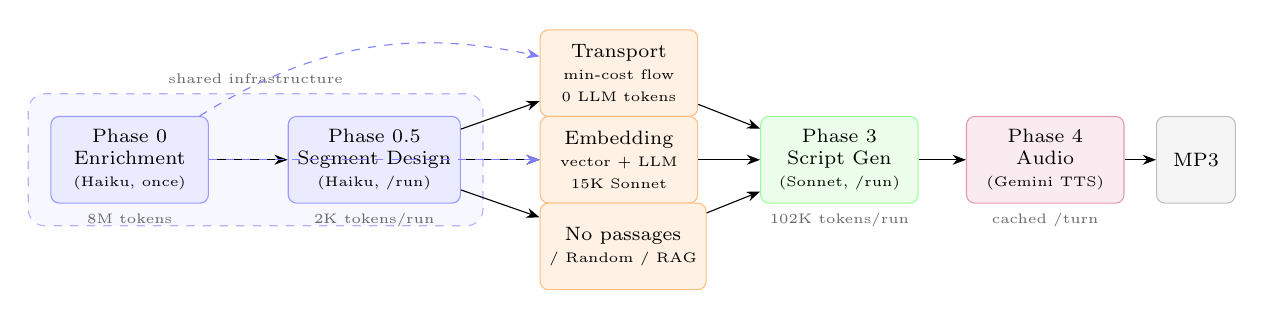
\begin{tikzpicture}[
    >=Stealth,
    phase/.style={draw, rounded corners=3pt, minimum height=1.1cm,
      minimum width=2.0cm, align=center, font=\scriptsize},
    shared/.style={phase, fill=blue!8, draw=blue!40},
    varies/.style={phase, fill=orange!10, draw=orange!50},
    fixed/.style={phase, fill=green!8, draw=green!40},
    annot/.style={font=\tiny, text=black!60},
    every edge/.style={->, thick, black!70},
  ]
  % Phase 0: Enrichment
  \node[shared] (enrich) {Phase 0\\Enrichment\\{\tiny (Haiku, once)}};
  \node[annot, below=0pt of enrich] {8M tokens};

  % Phase 0.5: Segment design
  \node[shared, right=1.0cm of enrich] (segment) {Phase 0.5\\Segment Design\\{\tiny (Haiku, /run)}};
  \node[annot, below=0pt of segment] {2K tokens/run};

  % Phase 1+2: Selection (three branches)
  \node[varies, right=1.0cm of segment, yshift=1.1cm] (transport)
    {Transport\\{\tiny min-cost flow}\\{\tiny 0 LLM tokens}};
  \node[varies, right=1.0cm of segment] (embedding)
    {Embedding\\{\tiny vector + LLM}\\{\tiny 15K Sonnet}};
  \node[varies, right=1.0cm of segment, yshift=-1.1cm] (nop)
    {No passages\\{\tiny / Random / RAG}};

  % Phase 3: Script generation
  \node[fixed, right=3.8cm of segment] (script)
    {Phase 3\\Script Gen\\{\tiny (Sonnet, /run)}};
  \node[annot, below=0pt of script] {102K tokens/run};

  % Phase 4: Audio rendering
  \node[phase, right=0.6cm of script, fill=purple!8, draw=purple!40]
    (audio) {Phase 4\\Audio\\{\tiny (Gemini TTS)}};
  \node[annot, below=0pt of audio] {cached /turn};

  % Output
  \node[phase, right=0.4cm of audio, fill=gray!8, draw=gray!50,
    minimum width=1.0cm]
    (output) {MP3};

  % Edges
  \draw[->] (enrich) -- (segment);
  \draw[->] (segment) -- (transport);
  \draw[->] (segment) -- (embedding);
  \draw[->] (segment) -- (nop);
  \draw[->] (transport) -- (script);
  \draw[->] (embedding) -- (script);
  \draw[->] (nop) -- (script);
  \draw[->] (script) -- (audio);
  \draw[->] (audio) -- (output);

  % Enrichment feeds selection
  \draw[->, dashed, blue!50] (enrich) to[bend left=22] (transport);
  \draw[->, dashed, blue!50] (enrich) to[bend left=0] (embedding);

  % Shared label
  \begin{scope}[on background layer]
    \node[draw=blue!30, dashed, rounded corners=6pt, fill=blue!3,
      fit=(enrich)(segment), inner sep=8pt,
      label={[annot,anchor=south]above:shared infrastructure}] {};
  \end{scope}
\end{tikzpicture}
\caption{Pipeline architecture.  The shared enrichment layer (blue,
  left) is computed once.  Passage selection (orange, centre) varies by
  condition---transport uses zero LLM tokens.  Script generation
  (green, right) is identical across conditions.  Dashed arrows show
  enrichment data flowing to selection.}
\label{fig:pipeline}
\end{figure*}


\subsection{Enrichment Layer}
\label{sec:enrichment}

Each novel is split into passages (one per paragraph or small group of
paragraphs) and each passage is annotated by an LLM (Haiku) with 20
structured fields: an interest score (0--5), seven provision dimensions
(character\_development, plot\_advancement, thematic\_depth,
social\_critique, humor\_entertainment, atmosphere\_setting,
narrative\_technique---each rated none/weak/strong as 0/1/2),
characters present, themes, emotional register, plot function,
quotability, and a best\_quote extraction.

\begin{table}[t]
\caption{Corpus statistics.  All five novels are enriched with the
  same 20-field schema; passage counts reflect natural paragraph
  boundaries.}
\label{tab:corpus}
\begin{tabular}{lrrr}
\toprule
Novel & Chapters & Passages & Year \\
\midrule
\textit{Bleak House} (Dickens)        & 67 & 6{,}916 & 1853 \\
\textit{Our Mutual Friend} (Dickens)  & 63 & 5{,}775 & 1865 \\
\textit{The Mill on the Floss} (Eliot) & 58 & 4{,}654 & 1860 \\
\textit{North and South} (Gaskell)    & 52 & 2{,}942 & 1855 \\
\textit{A Passage to India} (Forster) & 37 & 2{,}556 & 1924 \\
\midrule
\textit{Total}                         & 277 & 22{,}843 & \\
\bottomrule
\end{tabular}
\end{table}

Table~\ref{tab:corpus} shows the five novels and their passage counts.
For the embedding pipeline, each passage also receives a contextual
retrieval summary \citep{anthropic2024context} prepended before
embedding with OpenAI \texttt{text-embedding-3-small}.  Total
enrichment cost across all five novels: ${\sim}$25M Haiku tokens plus
${\sim}$4.5M OpenAI embedding tokens, amortised across all runs at zero
marginal cost.


\subsection{Expert Personas and Demand Profiles}
\label{sec:personas}

Six expert personas, three per episode: \textbf{Hartley} (literary
critic), \textbf{Blackstone} (legal historian), \textbf{Woodcourt}
(close reader), \textbf{Edmund} (traditionalist), \textbf{Rosen}
(Marxist critic), \textbf{Trevelyan} (performer).  Each has a
\emph{demand profile}: a vector over the seven provision dimensions.
These are the primary editorial control surface
(Figure~\ref{fig:demand}).

\begin{figure}[t]
\centering
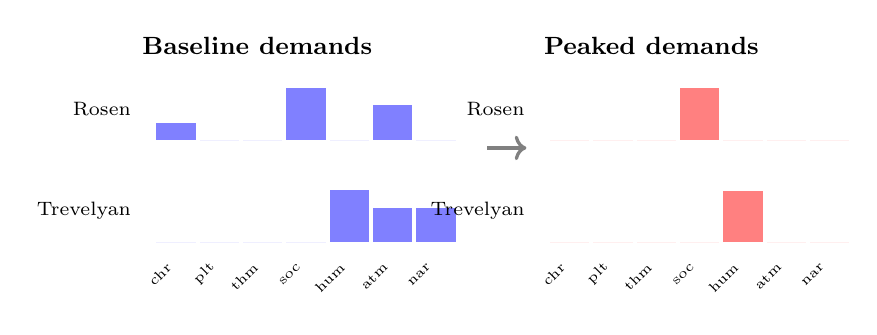
\begin{tikzpicture}[
    font=\scriptsize,
    bar/.style={fill=#1, draw=#1!80, minimum height=3pt},
  ]
  \def\dw{0.55}  % bar width
  \def\dlabels{{"chr","plt","thm","soc","hum","atm","nar"}}

  % --- Baseline ---
  \node[font=\small\bfseries, anchor=west] at (-0.3, 2.8) {Baseline demands};
  % Rosen baseline: social=3, atmos=2, char=1
  \node[anchor=east, font=\scriptsize] at (-0.2, 2.0) {Rosen};
  \foreach \v/\i in {1/0, 0/1, 0/2, 3/3, 0/4, 2/5, 0/6} {
    \fill[blue!50] (\i*\dw, 1.6) rectangle +(\dw-0.05, \v*0.22);
  }
  % Trevelyan baseline: humor=3, atmos=2, narr=2
  \node[anchor=east, font=\scriptsize] at (-0.2, 0.7) {Trevelyan};
  \foreach \v/\i in {0/0, 0/1, 0/2, 0/3, 3/4, 2/5, 2/6} {
    \fill[blue!50] (\i*\dw, 0.3) rectangle +(\dw-0.05, \v*0.22);
  }
  % Dimension labels (manual to avoid pgfmathparse string issues)
  \foreach \lab/\i in {chr/0, plt/1, thm/2, soc/3, hum/4, atm/5, nar/6} {
    \node[rotate=45, anchor=east, font=\tiny] at (\i*\dw+0.25, 0.1) {\lab};
  }

  % --- Peaked ---
  \node[font=\small\bfseries, anchor=west] at (4.8, 2.8) {Peaked demands};
  \def\ox{5.0}
  % Rosen peaked: social=8
  \node[anchor=east, font=\scriptsize] at (\ox-0.2, 2.0) {Rosen};
  \foreach \v/\i in {0/0, 0/1, 0/2, 8/3, 0/4, 0/5, 0/6} {
    \fill[red!50] (\ox+\i*\dw, 1.6) rectangle +(\dw-0.05, \v*0.082);
  }
  % Trevelyan peaked: humor=8
  \node[anchor=east, font=\scriptsize] at (\ox-0.2, 0.7) {Trevelyan};
  \foreach \v/\i in {0/0, 0/1, 0/2, 0/3, 8/4, 0/5, 0/6} {
    \fill[red!50] (\ox+\i*\dw, 0.3) rectangle +(\dw-0.05, \v*0.082);
  }
  % Dimension labels
  \foreach \lab/\i in {chr/0, plt/1, thm/2, soc/3, hum/4, atm/5, nar/6} {
    \node[rotate=45, anchor=east, font=\tiny] at (\ox+\i*\dw+0.25, 0.1) {\lab};
  }

  % Arrow between
  \draw[->, very thick, black!50] (4.2, 1.5) -- (4.7, 1.5);
\end{tikzpicture}
\caption{Demand profile manipulation.  Left: baseline demands are
  spread across dimensions.  Right: peaked demands concentrate each
  expert on their defining dimension (Rosen $\to$ 100\%
  social\_critique, Trevelyan $\to$ 100\% humor).  The transport solver
  responds by selecting qualitatively different passages (Jaccard 0.490
  with baseline).}
\label{fig:demand}
\end{figure}


\subsection{Min-Cost Flow Formulation}
\label{sec:transport}

Passage selection is a min-cost flow problem on a bipartite graph
(Figure~\ref{fig:flow}).  Supply nodes represent passages; demand
nodes represent expert--dimension pairs.  Edge costs encode quality
preference (strong provisions cost 1, weak cost 3), interest bonus
(passages scoring 4--5 get a cost reduction), a cluster penalty
$\lambda \cdot (k - 1)$ for chapter-level diversity, and a null cost
of 100 for unmet demand.

\begin{figure}[t]
\centering
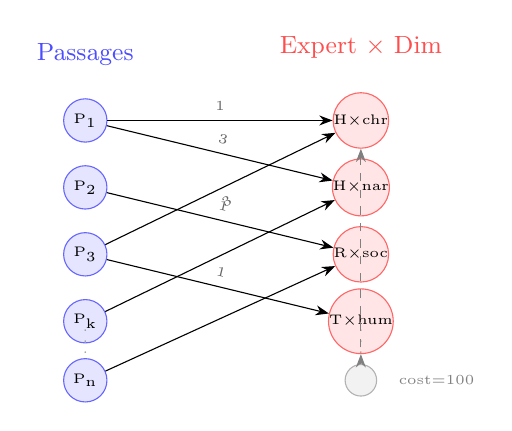
\begin{tikzpicture}[
    >=Stealth,
    node distance=0.5cm,
    supply/.style={circle, draw=blue!60, fill=blue!10,
      minimum size=0.55cm, font=\tiny, inner sep=0pt},
    demand/.style={circle, draw=red!60, fill=red!10,
      minimum size=0.55cm, font=\tiny, inner sep=0pt},
    null/.style={circle, draw=gray!60, fill=gray!10,
      minimum size=0.4cm, font=\tiny, inner sep=0pt},
    every edge/.style={->, thin, black!40},
    costlabel/.style={font=\tiny, text=black!60, midway},
  ]
  % Supply nodes (passages)
  \foreach \i/\lab in {1/P\textsubscript{1},2/P\textsubscript{2},
    3/P\textsubscript{3},4/P\textsubscript{k}} {
    \node[supply] (s\i) at (0, -\i*0.85+0.85) {\lab};
  }
  \node[font=\tiny, text=black!40] at (0, -2.7) {$\vdots$};
  \node[supply] (s5) at (0, -3.3) {P\textsubscript{n}};

  % Demand nodes (expert x dimension)
  \foreach \i/\lab in {1/{H$\times$chr},2/{H$\times$nar},
    3/{R$\times$soc},4/{T$\times$hum}} {
    \node[demand] (d\i) at (3.5, -\i*0.85+0.85) {\lab};
  }
  \node[font=\tiny, text=black!40] at (3.5, -2.7) {$\vdots$};

  % Null node
  \node[null] (nulln) at (3.5, -3.3) {$\varnothing$};

  % Edges with cost labels
  \draw[->] (s1) -- node[costlabel, above, sloped] {1} (d1);
  \draw[->] (s1) -- node[costlabel, above, sloped] {3} (d2);
  \draw[->] (s2) -- node[costlabel, above, sloped] {1} (d3);
  \draw[->] (s3) -- node[costlabel, above, sloped] {1} (d4);
  \draw[->] (s3) -- node[costlabel, below, sloped] {3} (d1);
  \draw[->] (s4) -- (d2);
  \draw[->] (s5) -- (d3);
  \draw[->, dashed, gray] (nulln) -- (d1);
  \draw[->, dashed, gray] (nulln) -- (d4);

  % Labels
  \node[font=\small, above=0.3cm of s1, text=blue!70] {Passages};
  \node[font=\small, above=0.3cm of d1, text=red!70] {Expert $\times$ Dim};
  \node[font=\tiny, right=0.15cm of nulln, text=gray] {cost=100};
\end{tikzpicture}
\caption{Bipartite flow graph.  Passages (left) supply flow to
  expert--dimension demand nodes (right).  Edge costs reflect provision
  strength and interest.  The null node (bottom right, cost=100) absorbs
  unmet demand.  The solver finds the minimum-cost assignment.}
\label{fig:flow}
\end{figure}

The solver (SciPy \texttt{min\_cost\_flow}) finds a global optimum
subject to capacity constraints.  A second min-cost flow assigns
selected passages to episode segments.  Because solving a flow is cheap
($<$1 second, zero LLM tokens), the user can adjust demand profiles and
re-solve interactively---the core of our manipulability hypothesis.

\subsection{Five Selection Conditions}
\label{sec:conditions}

All conditions share the same segment design (Phase~0, Haiku) and
script generation (Phase~3, Sonnet).  They differ only in what
passages are provided to Phase~3:

\begin{enumerate}
\item \textbf{No passages}: the LLM generates from prior knowledge
  alone.
\item \textbf{Random}: 32 passages sampled uniformly, assigned
  round-robin.
\item \textbf{Plain RAG}: top-$k$ passages by cosine similarity
  between expert persona embeddings and raw passage text.
\item \textbf{Embedding + LLM curation}: contextual embeddings
  \citep{anthropic2024context} with Sonnet chain-of-thought
  curation ($\sim$15K tokens per run).
\item \textbf{Transport}: min-cost flow over enrichment features
  (0 LLM tokens for selection).
\end{enumerate}


\subsection{Audio Rendering (Phase~4)}
\label{sec:audio}

The structured script is rendered to audio using Google's Gemini 2.5
TTS models (\texttt{gemini-2.5-flash-preview-tts} or
\texttt{gemini-2.5-pro-preview-tts}).  The separation of script
generation (Phase~3) from audio rendering (Phase~4) is deliberate:
the structured output schema carries enough annotation to drive TTS
without further LLM inference, and cached audio segments survive
script iteration.

Each speaker is assigned a distinct Gemini voice (e.g., Sulafat for
the host, Zephyr for Hartley, Gacrux for Blackstone) with an accent
direction embedded as a natural-language stage direction in the TTS
prompt (``Home Counties accent, BBC Radio~4 style'' for the host;
``Edinburgh accent, dry and authoritative'' for Blackstone).

The utterance-level annotations from Phase~3---rate multiplier, pause
timing, emphasis words, and quote mode---are translated into
natural-language prosody directions rather than SSML parameters:

\begin{itemize}
\item \textbf{Rate}: a multiplier of 0.93 becomes ``Speak slowly and
  deliberately''; 1.04 becomes ``Speak with brisk energy.''
\item \textbf{Quote mode}: ``setup'' $\to$ ``Build anticipation---this
  leads into a literary quotation''; ``reading'' $\to$ ``Read this as
  a direct literary quotation with weight and relish.''
\item \textbf{Pauses}: \texttt{pause\_before\_ms} and
  \texttt{pause\_after\_ms} are realised as synthesised silence
  segments inserted during post-processing, not via TTS timing.
\item \textbf{Emphasis}: up to 3 words per utterance, passed as
  ``Give slight emphasis to: \emph{Chancery}, \emph{fog}.''
\end{itemize}

Figure~\ref{fig:tts} illustrates the rendering pipeline for a single
turn.

\begin{figure}[t]
\centering
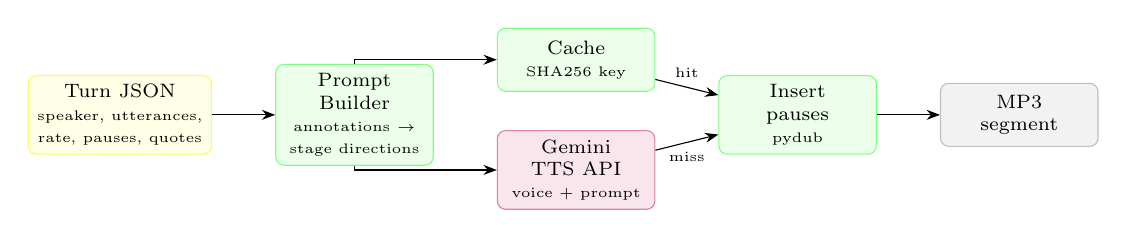
\begin{tikzpicture}[
    >=Stealth,
    font=\scriptsize,
    box/.style={draw, rounded corners=3pt, minimum height=0.8cm,
      align=center, minimum width=2.0cm},
    data/.style={box, fill=yellow!10, draw=yellow!60},
    proc/.style={box, fill=green!8, draw=green!50},
    api/.style={box, fill=purple!10, draw=purple!50},
    outfile/.style={box, fill=gray!10, draw=gray!50},
  ]
  % Input
  \node[data] (turn) at (0, 0) {Turn JSON\\{\tiny speaker, utterances,}\\{\tiny rate, pauses, quotes}};

  % Prompt builder
  \node[proc, right=0.8cm of turn] (prompt) {Prompt\\Builder\\{\tiny annotations $\to$}\\{\tiny stage directions}};

  % Cache check
  \node[proc, right=0.8cm of prompt, yshift=0.7cm] (cache) {Cache\\{\tiny SHA256 key}};
  \node[api, right=0.8cm of prompt, yshift=-0.7cm] (gemini) {Gemini\\TTS API\\{\tiny voice + prompt}};

  % Post-process
  \node[proc, right=0.8cm of cache, yshift=-0.7cm] (post) {Insert\\pauses\\{\tiny pydub}};

  % Output
  \node[outfile, right=0.8cm of post] (mp3) {MP3\\segment};

  % Edges
  \draw[->] (turn) -- (prompt);
  \draw[->] (prompt) |- (cache);
  \draw[->] (prompt) |- (gemini);
  \draw[->] (cache) -- node[above, font=\tiny] {hit} (post);
  \draw[->] (gemini) -- node[below, font=\tiny] {miss} (post);
  \draw[->] (post) -- (mp3);
\end{tikzpicture}
\caption{Audio rendering pipeline (Phase~4).  Utterance annotations
  from Phase~3 are translated to natural-language stage directions.
  Rendered turns are cached by content hash; pauses are inserted in
  post-processing.  Output is MP3 at 24\,kHz mono.}
\label{fig:tts}
\end{figure}

Rendered audio is cached per turn (keyed by SHA-256 hash of model,
voice, and prompt text), so re-rendering after script edits only
re-synthesises changed turns.  Final output is 24\,kHz mono MP3.
Phase~4 is not part of the experimental comparison---all five
conditions use the same rendering pipeline---but the structured
annotations it consumes are a design constraint on Phase~3's output
schema, and the natural-language prosody directions demonstrate that
the utterance-level annotations (rate, quote mode, pauses) carry
meaningful information beyond text.


\section{Experimental Design}
\label{sec:experiment}

For \textit{Bleak House}, all $\binom{6}{3} = 20$ possible three-expert
panels are run under all five conditions: 100 episodes.  For each of
the other four novels, 8 panels are run under three conditions
(transport, embedding, no-passages): 96 episodes.  The total is 196
episodes across five novels.  Across all conditions and novels:
identical segment design, identical script generation prompt, identical
persona descriptions, identical Pydantic output schema.  The only
manipulation is what appears in the ``Assigned Passages'' section of
the Phase~3 prompt.

\textbf{Metrics.}  Character mention density (per 1{,}000 words,
against each novel's named character list), character entropy
\citep{shannon1948mathematical}, unique characters per episode, quotes
per episode, per-expert TF-IDF vocabulary signatures (cross-condition
and cross-novel cosine), quote verification (fuzzy 5-word subsequence
matching against source text), and material similarity (Jaccard,
Jensen-Shannon divergence \citep{lin1991divergence}, maximum mean
discrepancy \citep{gretton2012kernel}).


\section{Results}
\label{sec:results}

\subsection{Hypothesis 1: Manipulability}
\label{sec:manipulability}

The central claim is that transport's demand profiles provide a
control surface that embedding-based retrieval lacks.  We test this
with two manipulation strategies applied to the transport pipeline
(Figure~\ref{fig:manipulability}).

\begin{figure}[t]
\centering
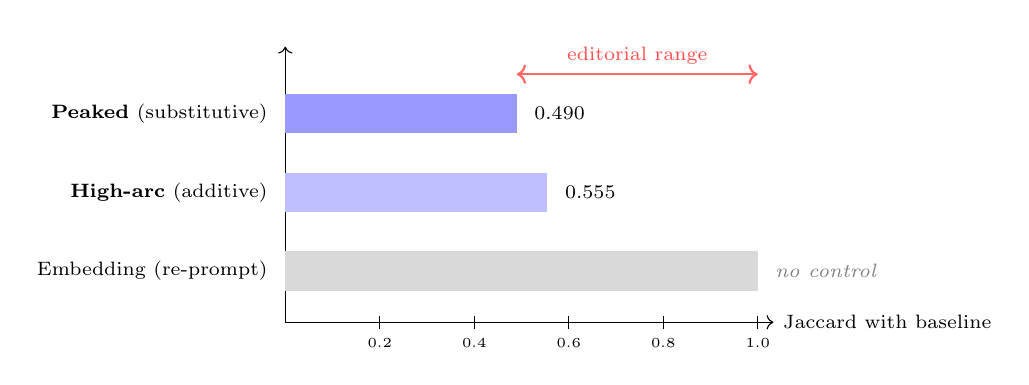
\begin{tikzpicture}[font=\small]
  % Axes
  \draw[->] (0,0) -- (6.2,0) node[right, font=\scriptsize] {Jaccard with baseline};
  \draw[->] (0,0) -- (0,3.5) node[above, font=\scriptsize] {};

  % Tick marks
  \foreach \x/\v in {1.2/0.2, 2.4/0.4, 3.6/0.6, 4.8/0.8, 6.0/1.0} {
    \draw (\x, -0.08) -- (\x, 0.08);
    \node[below, font=\tiny] at (\x, -0.08) {\v};
  }

  % Bars
  \fill[blue!40] (0, 2.4) rectangle (2.94, 2.9)  % 0.490 * 6
    node[midway, font=\scriptsize, text=white] {};
  \node[anchor=east, font=\scriptsize] at (-0.1, 2.65)
    {\textbf{Peaked} (substitutive)};
  \node[anchor=west, font=\scriptsize] at (3.04, 2.65) {0.490};

  \fill[blue!25] (0, 1.4) rectangle (3.33, 1.9)  % 0.555 * 6
    node[midway, font=\scriptsize, text=white] {};
  \node[anchor=east, font=\scriptsize] at (-0.1, 1.65)
    {\textbf{High-arc} (additive)};
  \node[anchor=west, font=\scriptsize] at (3.43, 1.65) {0.555};

  \fill[gray!30] (0, 0.4) rectangle (6.0, 0.9);
  \node[anchor=east, font=\scriptsize] at (-0.1, 0.65)
    {Embedding (re-prompt)};
  \node[anchor=west, font=\scriptsize, text=black!50] at (6.1, 0.65)
    {\textit{no control}};

  % Annotation
  \draw[<->, thick, red!60] (2.94, 3.15) -- (6.0, 3.15);
  \node[above, font=\scriptsize, red!70] at (4.47, 3.15)
    {editorial range};
\end{tikzpicture}
\caption{Manipulability comparison.  Transport demand changes produce
  measurably different passage sets (Jaccard 0.490--0.555 with
  baseline).  The embedding pipeline has no equivalent parameter; the
  user must re-prompt the LLM curator with no guarantee of systematic
  change.}
\label{fig:manipulability}
\end{figure}

\textbf{Additive (high-arc).}  Doubling character arc demands adds
exactly 15 passages per panel (matching the extra demand units),
producing Jaccard overlap 0.555 with the baseline.  Character mentions
increase (Richard $+$30\%, Jo $+$11\%) but the podcast is
qualitatively unchanged.  The manipulation is \emph{predictable}:
added passages trace directly to added demand units.

\textbf{Substitutive (peaked).}  Peaking each expert's demand vector
---amplifying the defining dimension while zeroing
secondaries---produces Jaccard overlap 0.490 (less than half the
passages are shared).  Rosen's passages become 100\% social\_critique
(vs 56\% at baseline); Trevelyan's become 100\% humor (vs 53\%).
Hartley's dominant dimension \emph{flips} from character\_development
to narrative\_technique.  The manipulation is \emph{transformative}:
it reshapes the editorial character of the episode.

The embedding pipeline has no equivalent mechanism.  The user cannot
express ``what if Rosen demands only social critique?'' as a retrieval
query.  The only recourse is to rewrite the curation prompt and hope
the LLM responds systematically.


\subsection{Hypothesis 2: Exploration Cost}
\label{sec:cost}

Figure~\ref{fig:cost} compares the token cost of exploring alternatives.

\begin{figure}[t]
\centering
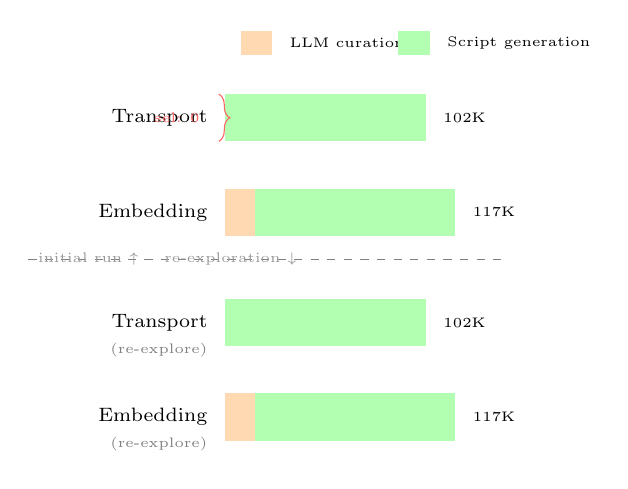
\begin{tikzpicture}[font=\small]
  % Cost comparison
  \def\bw{0.6}
  \def\scl{0.025}  % scale: 1K tokens = 0.025cm

  % Transport
  \node[anchor=east, font=\scriptsize] at (-0.1, 2.5) {Transport};
  % Script gen only (102K)
  \fill[green!30] (0, 2.2) rectangle (102*\scl, 2.8);
  \node[font=\tiny, anchor=west] at (102*\scl+0.1, 2.5) {102K};

  % Embedding
  \node[anchor=east, font=\scriptsize] at (-0.1, 1.3) {Embedding};
  % Curation (15K) + Script gen (102K) = 117K
  \fill[orange!30] (0, 1.0) rectangle (15*\scl, 1.6);
  \fill[green!30] (15*\scl, 1.0) rectangle (117*\scl, 1.6);
  \node[font=\tiny, anchor=west] at (117*\scl+0.1, 1.3) {117K};

  % Re-explore transport (just re-solve + script gen)
  \node[anchor=east, font=\scriptsize] at (-0.1, -0.1)
    {Transport};
  \node[anchor=east, font=\tiny, text=black!50] at (-0.1, -0.45)
    {(re-explore)};
  \fill[green!30] (0, -0.4) rectangle (102*\scl, 0.2);
  \node[font=\tiny, anchor=west] at (102*\scl+0.1, -0.1) {102K};

  % Re-explore embedding (re-curate + script gen)
  \node[anchor=east, font=\scriptsize] at (-0.1, -1.3)
    {Embedding};
  \node[anchor=east, font=\tiny, text=black!50] at (-0.1, -1.65)
    {(re-explore)};
  \fill[orange!30] (0, -1.6) rectangle (15*\scl, -1.0);
  \fill[green!30] (15*\scl, -1.6) rectangle (117*\scl, -1.0);
  \node[font=\tiny, anchor=west] at (117*\scl+0.1, -1.3) {117K};

  % Legend
  \fill[orange!30] (0.2, 3.3) rectangle (0.6, 3.6);
  \node[anchor=west, font=\tiny] at (0.7, 3.45) {LLM curation};
  \fill[green!30] (2.2, 3.3) rectangle (2.6, 3.6);
  \node[anchor=west, font=\tiny] at (2.7, 3.45) {Script generation};

  % Divider
  \draw[dashed, gray] (-2.5, 0.7) -- (3.5, 0.7);
  \node[font=\tiny, text=black!40, anchor=west] at (-2.5, 0.7)
    {initial run $\uparrow$ \quad re-exploration $\downarrow$};

  % Brace: transport selection = 0
  \draw[decorate, decoration={brace, amplitude=4pt, mirror}, red!60]
    (-0.08, 2.2) -- (-0.08, 2.8);
  \node[font=\tiny, text=red!60, anchor=east] at (-0.2, 2.5) {sel: 0};
\end{tikzpicture}
\caption{Token cost per run.  Transport selection costs zero LLM
  tokens (red brace); embedding requires $\sim$15K Sonnet tokens for
  curation (orange).  Script generation (green) dominates both.  For
  re-exploration, transport re-solves instantly; embedding must
  re-prompt the curator.  Over $N$ explorations, transport saves $N
  \times 15$K Sonnet tokens.}
\label{fig:cost}
\end{figure}

The transport solver reads enrichment features as numeric vectors
---zero LLM tokens for selection.  The embedding pipeline requires
$\sim$15K Sonnet tokens per run for LLM curation.  Script generation
($\sim$102K tokens) dominates both, so the per-run saving is modest
(13\%).  But the cost advantage compounds with exploration: $N$
alternative configurations cost $N \times 102$K for transport vs
$N \times 117$K for embedding.  More importantly, transport
re-exploration requires only re-solving ($<$1s) before committing to
the expensive script generation step---the user can preview passage
assignments, evaluate them, and decide whether to generate a script.
The embedding pipeline offers no such preview.

Table~\ref{tab:cost} shows the full token budget.

\begin{table}[t]
\caption{Token budget by model class.  Enrichment is computed once per
  novel; per-run costs are dominated by script generation.}
\label{tab:cost}
\begin{tabular}{lrr}
\toprule
Component & Haiku & Sonnet \\
\midrule
Enrichment (once, 5 novels)   & 25M & --- \\
Segment design (/run)  & 2K & --- \\
Curation (/run, embed only) & --- & 15K \\
Script generation (/run) & --- & 102K \\
\midrule
Project total (196 runs) & 25.4M & 20.0M \\
\bottomrule
\end{tabular}
\end{table}

The enrichment layer's 25M Haiku tokens (across five novels) are
amortised across all runs.  Adding a new panel for one novel costs
$\sim$300K Sonnet tokens (3 conditions $\times$ $\sim$100K each).


\subsection{Aggregate Quality Comparison}
\label{sec:aggregate}

Table~\ref{tab:aggregate} shows that across all five novels, the
selection conditions produce comparable scripts on surface metrics.  The
\textit{Bleak House} results (all five conditions, 20 panels) and the
four-novel results (three conditions, 8 panels each) tell the same
story.

\begin{table}[t]
\caption{Aggregate metrics.  BH: 20 panels $\times$ 5 conditions.
  Cross-novel (XN): 4 novels $\times$ 8 panels $\times$ 3 conditions.}
\label{tab:aggregate}
\begin{tabular}{lrrrrr}
\toprule
Metric & Trns & Emb & RAG & NoPsg & Rnd \\
\midrule
Words/ep    & 9.3K & 10.0K & 9.4K & 10.6K & 8.6K \\
Quotes/ep   & 40.8 & 43.8 & 37.7 & 41.2 & 33.6 \\
Char/1Kw    & 22.3 & 17.6 & 23.1 & 23.8 & 22.1 \\
Uniq chars  & 14.4 & 11.6 & 16.2 & 16.0 & 18.5 \\
Char entropy & 3.43 & 2.91 & 3.48 & 3.28 & 3.71 \\
\bottomrule
\end{tabular}
\end{table}

Embedding narrows: lowest character density (17.6/1Kw), fewest unique
characters (11.6), lowest entropy (2.91) despite highest word count.
Plain RAG matches transport within 3\% on all metrics.  No passages
achieves 80\% of transport's character density from prior knowledge
alone.  These patterns hold across all five novels, confirming that
selection method has modest impact on aggregate quality---the persona
layer dominates.


\subsection{Passage Grounding Prevents Confabulation}
\label{sec:grounding}

\begin{table}[t]
\caption{Quote verification rates (fuzzy 5-word subsequence match).
  Top: \textit{Bleak House} (all 5 conditions).  Bottom: cross-novel
  means (3 conditions).}
\label{tab:quotes}
\begin{tabular}{lrr}
\toprule
Condition & Raw & Adjusted \\
\midrule
\multicolumn{3}{l}{\textit{Bleak House (5 conditions, 20 panels):}} \\
Transport       & 87\% & 91\% \\
Embedding       & 89\% & 96\% \\
Plain RAG       & 78\% & 91\% \\
No passages     & 38\% & 52\% \\
Random          & 65\% & --- \\
\midrule
\multicolumn{3}{l}{\textit{Cross-novel mean (3 conditions, 4 novels):}} \\
Transport       & 62\% & --- \\
Embedding       & 58\% & --- \\
No passages     & 10\% & --- \\
\bottomrule
\end{tabular}
\end{table}

The gap between no-passages and any grounded condition dwarfs the gap
between grounding methods.  This holds across all five novels
(Table~\ref{tab:quotes-xnovel}): the cross-novel grounding gap averages
+50 percentage points, ranging from +46 (Forster) to +59 (Gaskell).
Passage grounding prevents confabulation; the method of grounding is
secondary.

\begin{table}[t]
\caption{Quote verification rates by novel (transport, embedding,
  no-passages).  The grounding gap is large and consistent.}
\label{tab:quotes-xnovel}
\begin{tabular}{lrrrc}
\toprule
Novel & Trn & Emb & NP & Gap \\
\midrule
\textit{Bleak House}       & 87\% & 89\% & 38\% & +50 \\
Our Mutual Friend  & 53\% & 62\% &  5\% & +53 \\
Mill on the Floss  & 58\% & 55\% &  9\% & +47 \\
North and South    & 66\% & 59\% &  4\% & +59 \\
A Passage to India & 73\% & 58\% & 20\% & +46 \\
\midrule
\textit{Mean}      & 67\% & 65\% & 15\% & +51 \\
\bottomrule
\end{tabular}
\end{table}

Forster's novel shows the highest no-passages verification rate (20\%),
while Gaskell's and Dickens's \textit{Our Mutual Friend} show the
lowest ($\leq$5\%).  We note this variation without claiming a specific
cause; possible factors include corpus size, the LLM's training
exposure, and the density of quotable prose.


\subsection{Material Disjointness and Script Convergence}
\label{sec:material}

Transport and embedding select almost entirely different passages, yet
scripts partially converge.  Table~\ref{tab:material} shows this
pattern for \textit{Bleak House}; Table~\ref{tab:material-xnovel} shows
it replicates across all five novels.

\begin{table}[t]
\caption{Material disjointness (top) vs script convergence (bottom)
  for \textit{Bleak House}, transport $\leftrightarrow$ embedding,
  per-expert averages.}
\label{tab:material}
\begin{tabular}{lr}
\toprule
\multicolumn{2}{l}{\textit{Passage-level disjointness:}} \\
Passage Jaccard & 0.047 \\
Chapter Jaccard & 0.074 \\
Character JSD & 0.518 \\
Theme JSD & 0.411 \\
\midrule
\multicolumn{2}{l}{\textit{Script-level convergence:}} \\
Vocabulary cosine (same expert) & 0.549 \\
Character mention Jaccard & 0.430 \\
Sentence specificity & 0.87 vs 0.87 \\
\bottomrule
\end{tabular}
\end{table}

\begin{table}[t]
\caption{Convergence paradox across all five novels.  Passage Jaccard
  is near-zero everywhere; vocabulary cosine is consistently moderate.}
\label{tab:material-xnovel}
\begin{tabular}{lrrrr}
\toprule
Novel & Pass.\ J & Ch.\ J & Prov.\ D & Vocab.\ cos \\
\midrule
\textit{Bleak House}    & 0.047 & 0.074 & ---   & 0.549 \\
Our Mutual Friend       & 0.066 & 0.262 & 0.597 & 0.632 \\
Mill on the Floss       & 0.026 & 0.192 & 0.834 & 0.658 \\
North and South         & 0.024 & 0.216 & 0.676 & 0.674 \\
A Passage to India      & 0.085 & 0.312 & 0.413 & 0.683 \\
\bottomrule
\end{tabular}
\end{table}

The convergence force is the expert persona.  The same expert
discussing different passages about the same novel arrives at
overlapping vocabulary because the persona constrains what the expert
\emph{says about} the material.  This is the convergence paradox:
different inputs, similar outputs---because the persona, not the
passage, dominates.  The pattern holds uniformly across novels of
different lengths, authors, and literary periods.


\subsection{Expert Identity Is Robust}
\label{sec:identity}

G2 log-likelihood keywords \citep{dunning1993accurate} are stable
across conditions: Blackstone's vocabulary centres on \emph{legal,
chancery, victorian}; Rosen's on \emph{system, class, power};
Trevelyan's on \emph{read, aloud, voice, rhythm}.  Clustering 5{,}888
turns confirms expert identity (adjusted Rand index 0.345) is a
stronger grouping factor than condition (0.281).

Cross-condition cosine: embedding $\leftrightarrow$ transport 0.44,
no-passages $\leftrightarrow$ transport 0.36, random
$\leftrightarrow$ transport 0.30.  Random disrupts identity
\emph{more} than no passages---irrelevant grounding text interferes
with the persona prompt.

Expert personas also maintain stable signatures \emph{across novels}
(Table~\ref{tab:xnovel-airtime}).  Airtime proportions vary by at most
1.4 percentage points (SD) across the four non-BH novels.  Cross-novel
vocabulary cosine averages 0.89 per expert, confirming that the persona
prompt---not the source material---dominates each expert's linguistic
fingerprint.

\begin{table}[t]
\caption{Expert airtime (\% of total expert words, transport condition)
  across novels.  Proportions are remarkably stable; the persona prompt
  dominates over source material.}
\label{tab:xnovel-airtime}
\begin{tabular}{lrrrrr}
\toprule
Expert & OMF & MoF & NaS & PtI & SD \\
\midrule
Blackstone & 25.2 & 23.6 & 21.8 & 24.5 & 1.4 \\
Woodcourt  & 19.3 & 19.8 & 20.1 & 19.3 & 0.4 \\
Hartley    & 17.5 & 19.6 & 19.1 & 19.2 & 0.9 \\
Rosen      & 16.1 & 16.6 & 17.3 & 16.2 & 0.5 \\
Leigh      & 12.1 & 12.3 & 12.0 & 12.8 & 0.4 \\
Trevelyan  &  9.8 &  8.1 &  9.7 &  7.9 & 1.0 \\
\bottomrule
\end{tabular}
\end{table}


\subsection{Conversational Design Compliance}
\label{sec:conversational}

The script generation prompt encodes eight measurable conversational
design features.  Across all 196 episodes:

\begin{table}[t]
\caption{Conversational design measurements (196 episodes).}
\label{tab:conversational}
\begin{tabular}{lr}
\toprule
Feature & Measurement \\
\midrule
Expert$\to$expert transitions & 68\% \\
Host turn fraction & 23.5\% \\
Quote pattern compliance & 74.9\% \\
Cross-expert passage refs & 61.4\% \\
TTS rate $\sigma$ & 0.027 \\
Reactive markers/episode & 18.7 \\
\bottomrule
\end{tabular}
\end{table}

Cross-expert passage referencing (61.4\%) is the strongest signal
that shared context produces genuine conversation, not parallel
monologues.


\section{Planned: Host Preparation (Phase~2.5)}
\label{sec:host-prep}

The weakest conversational metric in Table~\ref{tab:conversational}
is question frequency: 1.7 questions per segment.  The host steers
with statements and transitions rather than questions, producing
discussion that flows but rarely probes.  We hypothesise that giving
the host a \emph{preparation stage}---structured interviews with each
expert before script generation---will increase question frequency,
improve cross-referencing, and produce more targeted conversational
steering.

\subsection{Design}

Phase~2.5 inserts two sub-stages between passage assignment (Phase~2)
and script generation (Phase~3), as shown in
Figure~\ref{fig:hostprep}.

\begin{figure}[t]
\centering
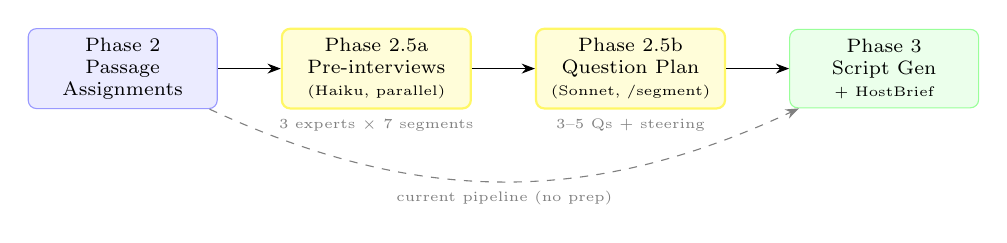
\begin{tikzpicture}[
    >=Stealth,
    font=\scriptsize,
    stage/.style={draw, rounded corners=3pt, minimum height=0.9cm,
      align=center, minimum width=2.4cm},
    input/.style={stage, fill=blue!8, draw=blue!40},
    new/.style={stage, fill=yellow!15, draw=yellow!60, thick},
    output/.style={stage, fill=green!8, draw=green!40},
    annot/.style={font=\tiny, text=black!50},
  ]
  % Input
  \node[input] (passages) at (0, 0) {Phase 2\\Passage\\Assignments};

  % Phase 2.5a: Pre-interviews
  \node[new, right=0.8cm of passages] (interview)
    {Phase 2.5a\\Pre-interviews\\{\tiny (Haiku, parallel)}};
  \node[annot, below=0pt of interview]
    {3 experts $\times$ 7 segments};

  % Phase 2.5b: Question planning
  \node[new, right=0.8cm of interview] (questions)
    {Phase 2.5b\\Question Plan\\{\tiny (Sonnet, /segment)}};
  \node[annot, below=0pt of questions]
    {3--5 Qs + steering};

  % Phase 3
  \node[output, right=0.8cm of questions] (script)
    {Phase 3\\Script Gen\\{\tiny + HostBrief}};

  % Edges
  \draw[->] (passages) -- (interview);
  \draw[->] (interview) -- (questions);
  \draw[->] (questions) -- (script);

  % Bypass arrow
  \draw[->, dashed, gray] (passages) to[bend right=25]
    node[below, annot] {current pipeline (no prep)} (script);
\end{tikzpicture}
\caption{Host preparation pipeline (Phase~2.5, planned).  Pre-interviews
  (Haiku, parallel per expert per segment) feed into question planning
  (Sonnet), producing a HostBrief that is injected into Phase~3.
  Dashed arrow shows the current pipeline without preparation.}
\label{fig:hostprep}
\end{figure}

\textbf{Phase~2.5a: Pre-interviews.}  For each expert--segment pair,
the host (Haiku) conducts a short interview: ``Given these passages,
what strikes you?  Where might you disagree with the other experts?
Which passage would you most want to quote?''  Each interview produces
a \texttt{PreInterviewResponse} (key points, potential quotes,
disagreement angles).  Calls are parallel ($\sim$22 per run: 3
experts $\times$ 7.5 segments), costing $\sim$1K Haiku tokens each.

\textbf{Phase~2.5b: Question planning.}  For each segment, the host
(Sonnet) synthesises all three experts' pre-interview responses and
plans 3--5 questions designed to: draw out each expert's strongest
take, set up productive disagreements, create cross-referencing
opportunities, and target specific passages for quotation.  Output is
a \texttt{HostBrief} (planned questions, steering notes,
cross-engagement targets).  One Sonnet call per segment ($\sim$3K
tokens each).

\textbf{Phase~3 integration.}  The HostBrief is appended to the
Phase~3 user message alongside the passage assignments.  The prompt
instructs: ``The host has prepared these questions---weave them
naturally into conversation, not as rigid Q\&A but as informed
steering.''

\subsection{Expected Cost}

Phase~2.5a: $\sim$22K Haiku tokens per run (parallel, cheap).
Phase~2.5b: $\sim$22K Sonnet tokens per run.  Total: $\sim$44K
additional tokens, a 43\% increase over the current per-run budget
but still dominated by Phase~3 script generation.

\subsection{Hypotheses and Planned Evaluation}

We will compare host-prepared vs unprepared episodes across at least 3
panels $\times$ 3 conditions (9+ paired comparisons):

\begin{enumerate}
\item \textbf{Question frequency} increases from 1.7 to 3--5 per
  segment.
\item \textbf{Cross-expert referencing} increases beyond the current
  61.4\%, as questions are designed to create cross-engagement.
\item \textbf{Reactive language markers} increase, as experts respond
  to targeted questions rather than free-associating.
\item \textbf{Quote pattern compliance} is maintained or improves, as
  the HostBrief targets specific passages for quotation.
\item \textbf{Expert identity} is not diluted---experts should still
  exhibit characteristic vocabulary despite more structured steering.
\end{enumerate}

\emph{Status: designed, data models and pipeline integration planned,
not yet implemented.}


\section{Planned: Conversational Prompt Ablation}
\label{sec:ablation}

The conversational design measurements in
Table~\ref{tab:conversational} show that the Phase~3 prompt's
instructions produce their intended effects.  But we do not yet know
which instructions are \emph{necessary}: does the model produce
expert-to-expert transitions because the prompt says ``this is a
conversation, not parallel monologues,'' or because the shared-context
architecture (all experts see all passages) makes cross-engagement
natural?  Does the three-part quote pattern emerge from the explicit
specification, or would the model structure quotes similarly without
it?

\subsection{Design}

We identify seven distinct conversational instructions in the Phase~3
system prompt and ablate each one individually, keeping passage
sharing and all other instructions intact.
Table~\ref{tab:ablation} lists the conditions and baseline
measurements.

\begin{table*}[t]
\caption{Prompt ablation conditions (planned).  Each condition removes
  one instruction from the Phase~3 system prompt.  Baseline
  measurements are from 233 episodes with all instructions present.}
\label{tab:ablation}
\begin{tabular}{llll}
\toprule
ID & Instruction removed & Baseline metric & Hypothesis \\
\midrule
A1 & ``Experts react to each other\ldots{} not & Expert$\to$expert 68\%,
  & Transitions become host- \\
   & \quad parallel monologues'' & cross-refs 61.4\%
  & \quad mediated; cross-refs drop \\
A2 & Quote setup$\to$reading$\to$commentary & Pattern compliance 74.9\%
  & Quotes appear but without \\
   & \quad pattern specification & & \quad consistent framing \\
A3 & Rate multiplier and pause & Rate $\sigma$=0.027,
  & Values collapse to 1.0 \\
   & \quad timing guidance & pause distributions
  & \quad or become erratic \\
A4 & Sentence type classification & 8-type distribution
  & Model defaults to \\
   & \quad requirement & (56\% analysis)
  & \quad ``analysis'' for most \\
A5 & ``At least one direct Dickens & 8.1\% quote\_reading
  & Quote frequency drops; \\
   & \quad quote per expert turn'' & utterances
  & \quad some turns ungrounded \\
A6 & Inter-speaker timing & pause\_before mean 221ms
  & Pauses lose context- \\
   & \quad guidance table & & \quad sensitivity \\
A7 & Host steering instructions & Host fraction 23.5\%
  & Host fraction changes \\
   & & & \quad unpredictably \\
\bottomrule
\end{tabular}
\end{table*}

Each ablation is run on the default panel (Hartley, Blackstone,
Woodcourt) with transport passages (v2 prompt), producing 7 ablated
episodes compared against the existing baseline.  Total cost: 7 runs
$\times$ $\sim$102K Sonnet tokens = $\sim$714K Sonnet tokens.

\subsection{Expected Findings}

The ablation study will classify each instruction into one of three
categories:

\begin{enumerate}
\item \textbf{Prompt-driven behaviours}: metrics that collapse when
  the instruction is removed.  We expect the three-part quote pattern
  (A2) and rate/pause guidance (A3) to be prompt-driven---the model
  has no reason to produce these specific patterns without instruction.
\item \textbf{Architecture-driven behaviours}: metrics that survive
  ablation because the shared-context architecture produces them
  naturally.  We hypothesise that cross-expert referencing (A1) may
  partially survive, since experts who see each other's passages have
  natural reason to engage with them regardless of the prompt
  instruction.
\item \textbf{Redundant instructions}: metrics that are unaffected
  because the model's default behaviour already matches the
  instruction.  Sentence type classification (A4) may be redundant if
  the model naturally produces functional variety in literary
  discussion.
\end{enumerate}

The most interesting potential finding is a dissociation between A1
and the cross-referencing metric: if removing ``experts react to each
other'' does \emph{not} reduce cross-referencing, then the
shared-passage architecture---not the prompt instruction---is the
active ingredient.  This would strengthen the system design argument
that passage sharing is the key architectural decision.

\emph{Status: ablation framework designed, 7 prompt variants and
analysis pipeline planned, not yet implemented.}




\section{Discussion}
\label{sec:discussion}

\subsection{Support for the Hypotheses}

\textbf{H1 (manipulability)}: confirmed.  Peaked demand vectors
produce Jaccard 0.490 with baseline, Rosen's dimension profile shifts
from 56\% to 100\% social\_critique, and Hartley's dominant dimension
flips.  These changes are predictable from the demand vector
adjustment, legible as flow changes, and impossible to replicate via
retrieval parameter tuning.

\textbf{H2 (exploration cost)}: confirmed for selection; attenuated
overall.  Transport selection costs zero tokens vs embedding's
$\sim$15K, a 13\% per-run saving.  But the real cost advantage is
\emph{preview without commitment}: the user can inspect passage
assignments before paying for script generation.

\subsection{Stereotypes as Editorial Objects}

The expert personas are deliberately stereotypical.  Following
\citet{boden2004creative}, the system performs combinational
creativity---but the interesting creativity is the user's, exploring
the configuration space and confronting the stereotypes that make the
machinery work.  Making stereotypes explicit as demand vectors, rather
than implicit in a prompt, turns editorial bias into a first-class
object that can be inspected, compared, and argued about.

\subsection{Limitations}

All evaluation is automated; no human listeners have judged the
generated episodes.  Statistical comparisons are descriptive; bootstrap
CIs would strengthen the claims.  The manipulability advantage assumes a
user who wants to explore configurations---for one-shot generation, the
transport pipeline offers no quality advantage over plain RAG.  The
five-novel study uses the same automated metrics throughout; human
evaluation remains future work.  All five novels are from the English
literary canon (1853--1924); the pipeline has not been tested on
non-literary text, non-English sources, or contemporary works.

\subsection{Implications}

Content selection for LLM-generated media need not be a retrieval
problem.  When source material is finite, pre-annotated, and
editorially constrained, combinatorial optimisation offers
inspectability, manipulability, and cheapness that retrieval cannot
match.  This applies beyond literary podcasts: legal document review,
curriculum design, exhibit curation---any setting where a user selects
content from a fixed corpus under competing priorities.


\begin{acknowledgments}
This work benefited from the infrastructure of LexisNexis Legal \&
Professional and conversations with colleagues at The Ohio State
University.  All experiments used the Anthropic and OpenAI APIs.
\end{acknowledgments}

\bibliographystyle{compling}
\bibliography{refs}

\end{document}
